%%%%%%%%%%%%%%%%%%%%%%%%%%%%%%
% 	   美赛模板,正文部分		 
%          PAPER.tex         
%%%%%%%%%%%%%%%%%%%%%%%%%%%%%%

\documentclass[11pt]{article}

% 请在此填写控制号、题号和标题,年份不需要填(自动以当前电脑时间年份为准)
\usepackage[1923231]{easymcm}\problem{C}   
\usepackage{palatino} % 这个是COMAP官方杂志采用的字体,如不需要可注释掉,以使用默认字体
\usepackage{subfigure}
\usepackage{float}
\usepackage{IEEEtrantools}
\captionsetup[figure]{font=scriptsize}
\title{\large God or evil? A ... model analysing and predicting opioid use}  % 标题
\setlength\parindent{0pt} %default no indent
\newcommand{\upcite}[1]{\textsuperscript{\textsuperscript{\cite{#1}}}}
\renewcommand{\figurename}{Fig.}
% 如您参加的是ICM(即选择了D/E/F题),请使用以下的命令修改Summary Sheet题头
% \renewcommand{\contest}{Interdisciplinary Contest in Modeling (ICM) Summary Sheet}

% 正文开始
\begin{document}
%%%%%%%%%%%%%%%%%%%%%%%%%%%%%%%%%%%%%%%%%
%%            请在此填写摘要            %%
%%%%%%%%%%%%%%%%%%%%%%%%%%%%%%%%%%%%%%%%%
\begin{abstract}\small
A non-SPA-style bathtub cannot be reheated by itself, so the water will get noticeably
cooler and users should add hot water from time to time. Based on the existing Partial
Differential Equation (PDE) technique, we construct time-space based temperature model
which can simulate any common condition. And then propose an optimal strategy
for users to keep the temperature even and close to initial temperature and decrease the
water consumption.

Firstly, we construct the PDE-solving model to simulate the temperature distribution
in the bathtub by analyzing the heat loss and confirming the corresponding parameters.
In this part, we consider two kinds of heat transfer, (water-bathtub heat conduction,
water-air heat convection), and the effect of inflow water on the faucet is shown by the
heat source. So we can confirm the boundary conditions of PDE to carry out the next
step.

Secondly, we do parameter testing by free cooling process to ensure the parameters
are in line with the actual condition. Most of the parameters are applicable, and a few
parameters are fine-tuned to make the model more accurate and practicable.
Thirdly, we confirm the optimal strategy by analyzing and comparing the continuous
and discontinuous flow methods, which vary from the temperature and flux. There are
two feasible methods gained from the analyses, one is continuous 42 $^\circ$C water inflow, the
other is turning on and off the faucet with 42 $^\circ$C inflow for 10 minutes.In addition, we
give two more kinds of methods.

At last, we use our model to determine the extent to which our strategy depends on
the factors of the bathtub, the factors of the user, and a bubble bath additive. And we test
the methods by changing the initial temperature. From those results, we further suggest
the users move less and use more bubble bath additive, and turning on the faucet at the
beginning is also a good choice.
\end{abstract}



%%%%%%%%%%%%%%%%%%%%%%%%%%%%%%%%%%%%%%%%%%
% 如不理解以下部分中各命令的含义,请勿修改! %
%%%%%%%%%%%%%%%%%%%%%%%%%%%%%%%%%%%%%%%%%%

%---------以下生成sheet页----------
% 下面的语句可调整全文行距为标准值的0.6倍,请自行使用
%\renewcommand{\baselinestretch}{0.6}\normalsize
\maketitle  % 生成sheet页
\thispagestyle{empty}   % 不要页眉页脚和页码
\setcounter{page}{-100} % 此命令仅是为了避免页码重复报错,不要在意

%---------以下生成目录----------
\newpage
\tableofcontents
\thispagestyle{empty}   % 不要页眉页脚和页码
\newpage

%---------以下生成正文----------
\setlength\parskip{0.8\baselineskip}  % 调整段间距
\setcounter{page}{1}    % 从正文开始计页码
\pagestyle{fancy}		% 摘要请到ABSTRACT.tex中填写

\section*{Memo}
\newpage

\section{Introduction}
\subsection{Problem Background}
Opioids, no matter synthetic ones or non-synthetic ones, play an significant role in our daily life. The proper utilization of opioids helps thousands of people get relieved from their pains. However, misuse of them can really destroy the society. Therefore, it is essential and urgent to gain a better understanding of opioids' spread and influencing factors.

Recent years have witnessed the tremendous growth of opioids cases. How this trend will develop remains an national concern. With data of annual drug use and socio-economic factors in five U.S. states over the past few years, we perform data mining and construct a model to figure out the pattern of opioids use and what contributes to it.

% \subsection{Literature Review}
% A literatrue\upcite{1} say something about this problem ...

\subsection{Our work}
We do such things ...

\begin{enumerate}[\bfseries 1.]
    \item We do ...
    \item We do ...
    \item We do ...
\end{enumerate}

\subsection{Assumptions}
Given the lack of data and limitation of our knowledge, we made the following assumption:
\begin{itemize}
    \item We assume that the data after processing is robust for futher use.
\end{itemize}

\section{Notations}
The primary notations used in this paper are listed in \textbf{Table \ref{tb:notation}}.
\begin{table}[!htbp]
\begin{center}
\caption{Notations}
\begin{tabular}{cl}
	\toprule
	\multicolumn{1}{m{3cm}}{\centering Symbol}
	&\multicolumn{1}{m{8cm}}{\centering Definition}\\
	\midrule
	$A$&the first one\\
	$b$&the second one\\
	$\alpha$ &the last one\\
	\bottomrule
\end{tabular}\label{tb:notation}
\end{center}
\end{table}

\section{Data Processing}
We are provided with two types of data, the number of drug reports in categories and socio-economic factors. Both of them are specific to counties. The original data contains a lot of redundant and invalid items, which can seriously affect the accuracy and versatility of our model. Thereby, we first apply some data processing techniques before we construct the model.

\subsection{Missing Data Processing}
% In US, each county is assigned a unique five-digit code called FIPS county code. 
In the worksheet about socio-economic factors, there are many cells that contain no valid information at all. We delete columns and rows which contains a lot of useless cells. For other columns and rows, when invalid items appear, we replace it with the average value of the entire sequence.

\subsection{Combine variables of a Socio-economic Factor}
For every year from 2010 to 2016, there are a list of variables about one single socio-economic factor. For instance, factor ANCERSTRY includes estimate, estimate margin of error, percent, etc. Those variables all reflect some information of the target factor in some aspects, hence how to rank their importance matters. 

In information theory, entropy represents the information a sequence contains\upcite{3}. So Entropy Weight Method (EWM), which gives each index a weight according to their entropy, is chosen to measure the significance of each index. Before that, we normalize the data given using the following equation.
\begin{equation}
	y_{i} = \frac{x_{i}-min(x_{i})}{max(x_{i}) - min(x_{i})}
\end{equation}
where $x_{i}$ and $y_{i}$ denotes the original sequence and processed sequence.

We apply EWM in the way addressed as follows (Using ANCERSTRY as an example):
\begin{itemize}
	\item Define Estimate, Estimate margin of error, Percent, Percent margin of error of ANCERSTRY is defined as $y_{j}$ ($y_{1}$ means Estimate...). Compute entropy for $y_{j}$: $ E_{j} = -\frac{\sum p_{i}lnp_{i}}{ln(n)}$, where $p_{i}=\frac{y_{ji}}{\sum_{i} y_{ji}}$, $E_{j}$ represents the entropy for each index.
	\item Compute weight for Estimate, Estimate margin of error, Percent, Percent margin of error of ANCERSTRY: $ W_{j} = \frac{E_{j}}{\sum E_{j}}$, where $W_{j}$ represents the weight for each index.
	\item Combine variables using the weight: $y'_{i} = \sum_{j} W_{j} * y_{ji}$
\end{itemize}
So far, we have combined several variables of a factor into one $y'_{i}$, and the same can be done to other factors. The newly generated sequence will be reserved for further analysis.

\subsection{Cluster Counties of Five States}
Since we have detailed number of drug reports, it is not hard to fit a curve to observe the trend of opioid use for each state and for each county. However, we consider this method inappropriate. On the one hand, the sample for only one county is normally fluctuating irregularly, i.e. drug reports of heroin in ACCOMACK, VA was 2, 38, 6 during 2012-2014. It is unnecessary and meaningless to bulid a model when facing such fluctuation. On the other hand, given the large number of all kinds of opioids, even one type change significantly, it is not obvious when viewed as the level of the whole state.

Considering that state and county are not suitable for our research, a unit in between is introduced. We put counties on a two-dimensional plane and regard them as nodes. Then, k-means clustering method\upcite{1}, which aims to partion nodes into $k$ clusters minimizing the within-cluster sum of squares, was performed. In our case, we take $k = 10$. The distance of two counties can be computed with their latitude and longtitude retrieved from U.S. Census Bureau\upcite{2}. The clusters we derived are labeled as Cluster-1, Cluster-2, ..., Cluster-10.
\begin{figure}[H]
	\centering
	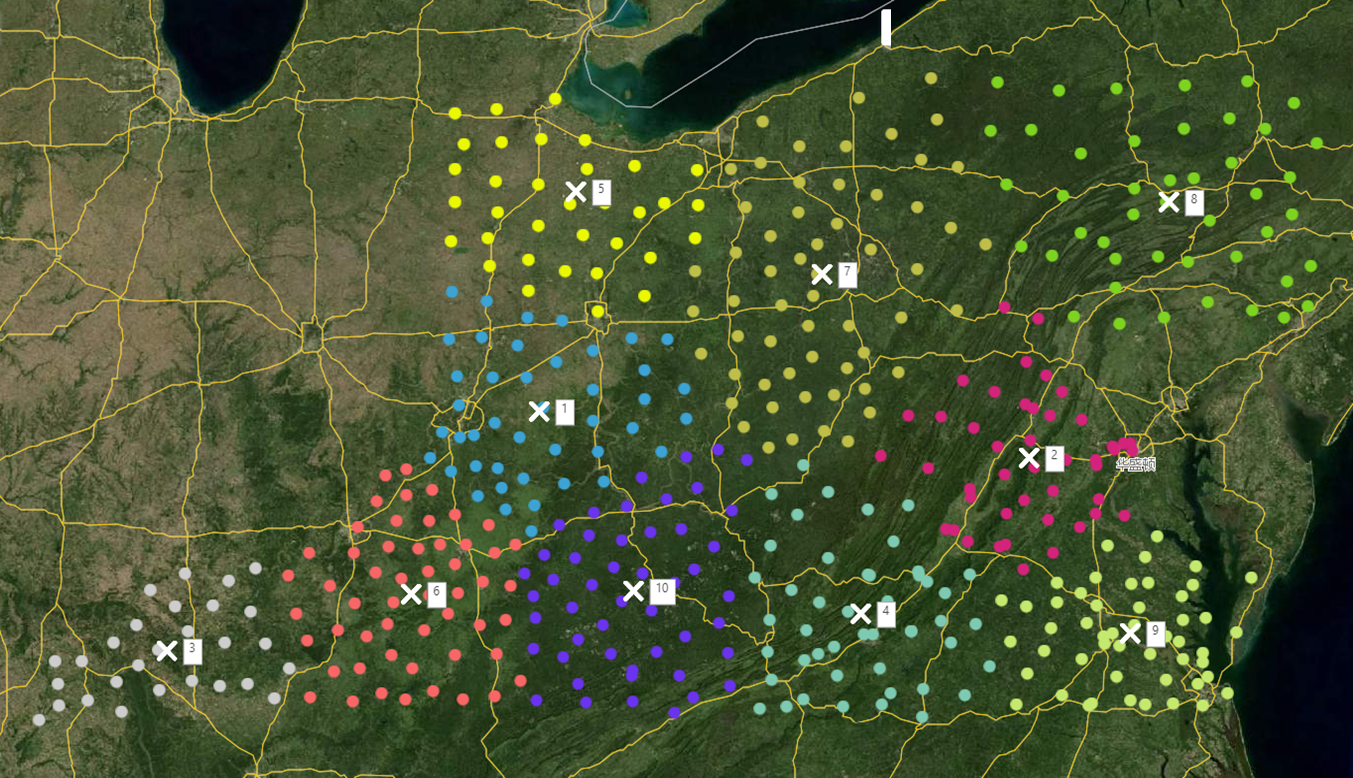
\includegraphics[scale=0.3]{./figures/0.png}
	\caption{Clusters got after k-means, points with the same color belong to one cluster}
	\label{Fig0}
\end{figure}

\subsection{Data Screening -- Drug Classification}
In order to describe the dissemination and characteristics of the synthetic opioids and heroin spread sperately, we need to screen the information in MCM\_NFLIS\_Data.xlsx. By consulting Wikipedia, DrugBank\upcite{4} and other websites, provided drugs are roughly classified into synthetic opioids, semi-synthetic opioids, and natural ingredients. In view of the topic requirements, we excluded the natural ingredients and drugs other than heroin in semi-synthetic opioids, leaving the drug reports of heroin and synthetic opioids only. As for the synthetic opioid, we find that many drugs have been used in small amounts over the years compared to those used in large numbers. And some drugs only start to appear in the past two years, so we can just ignore them. Finally, we leave about 15 kinds of synthetic drugs that have appeared since 2010 for further research.

\section{Model Construction}
\subsection{Identify Locations using Logistic Regression}
\subsubsection{Model Establishment}
With the K-means cluster analysis, we acquire data about the synthetic opioid and heroin events in ten clusters. It is clear to identify that the drug use levels in most areas are increasing. If drug use continues to grow at such speed, it will bring about numerous negative effects to the society when it exceeds an certain level, as mentioned in the Problem Background. Therefore, government’s relevant departments, including the Drug Enforcement Administration(DEA), will take corresponding measures to control the growing trend of drug use. However, when consumptions reach a high level, the growing rate in usage will reduce. And it is gradually increasing when consumptions are low.

This regular drug-use pattern is consistent with the Logistic model of population growth, in which the natural growth rate of the population will be limited by the population. Similarly, the drug-use will be limited by many restrictions including social factors such as government control and natural factors such as population growth. Assuming that drug-use level could be affected by these factors and thus having a ceiling, it can be considered that the growth trend of synthetic opioid and heroin events are subordinated to the Logistic model. Here’s the Logistic model:
\begin{equation}
	\begin{split}
	\frac{dN(t)}{dt} = r&(1-\frac{N(t)}{K})N(t) \label{logistic}\\
	N(t_{0}) &= N_{0}
	\end{split}
\end{equation}

where $N(t)$ represents the drug-use amount time $t$, $K$ represents the upper bound of the drug-use level and $r$ means an influence factor of the drug-use amount. Here we choose $r=1$. The model can be understood that there is no strict control and the drug is attractive in the early time, which results in the quickly increase of the drug use. As some departments begin to pay attention to this phenomenon and implement policies to control it, the growth rate of drug use begins to decrease. When the drug-use level is close to the allowable upper bound, $\frac{(1-Q)}{K} \approx 0$ . At this point, the drug-use level will no longer increase. Considering that our model is discrete in time,  we replace $\frac{dN(t)}{dt}$ with $N(t+1)-N(t)$.

The following equations gives the solution of logistic regression (Equation (\ref{logistic})).
\begin{gather}
	N(t)=\frac{K}{1+Ce^{-(t-t_{0})}} \\
	C=\frac{K-N_{0}}{N_{0}} 
\end{gather}
The above mathematical formulas and model can be established by programing. We utilize the data of ten clusters to buildthe model and acquire the logistic regressing curves.

\subsubsection{Model Application and Solving Problems}
In order to test the effectiveness of our model, we first put the total drug reports into the model for regressing and fitting, and get the following results. From the above clusters mentioned, the drug-use level in some areas is decreasing or fluctuating, we find three unsuitable clusters(Cluster-4, Cluster-5, Cluster-10) and the Fig. \ref{Fig.1} can show that those data are not suitable in this model. Therefore we cannot use the Logistic population growth model to perform regression of these areas’ drug reports. That is to say, other models may be needed for their prediction, which is not considered currently.

\begin{figure}[H]
	\centering %图片全局居中
	%并排几个图,就要写几个minipage
	\begin{minipage}[b]{0.45\textwidth} %所有minipage宽度之和要小于1,否则会自动变成竖排
		\centering %图片局部居中
		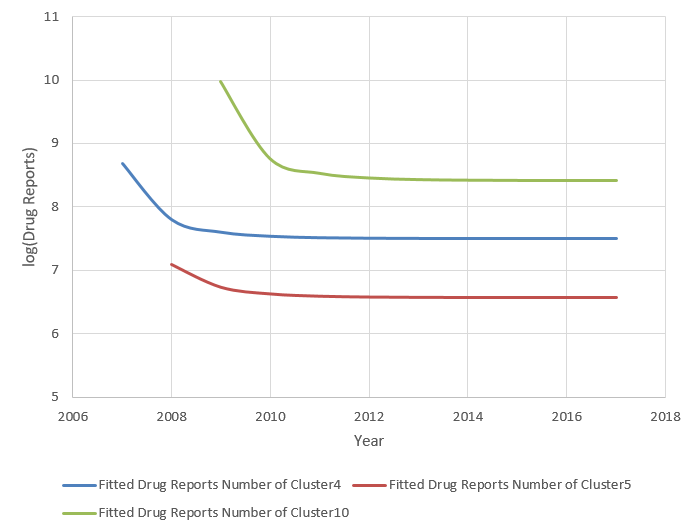
\includegraphics[scale=0.39]{./figures/1.png} %此时的图片宽度比例是相对于这个minipage的,不是全局
		\caption{Total Drug Reports Curves of Unsuitable Clusters}
		\label{Fig.1}
	\end{minipage}
	\begin{minipage}[b]{0.45\textwidth} %所有minipage宽度之和要小于1,否则会自动变成竖排
		\centering %图片局部居中
		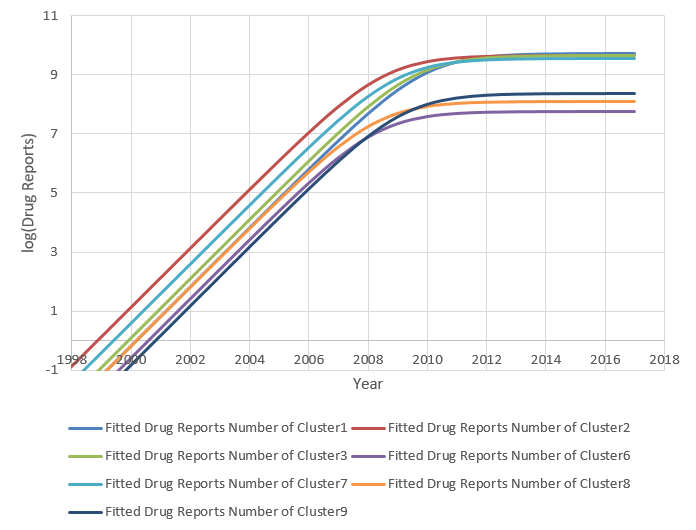
\includegraphics[scale=0.4]{./figures/2.png}%此时的图片宽度比例是相对于这个minipage的,不是全局
		\caption{Total Drug Reports Curves of Suitable Clusters}
		\label{Fig.2}
	\end{minipage}
\end{figure}

% \begin{figure}[H]
% 	\centering
% 	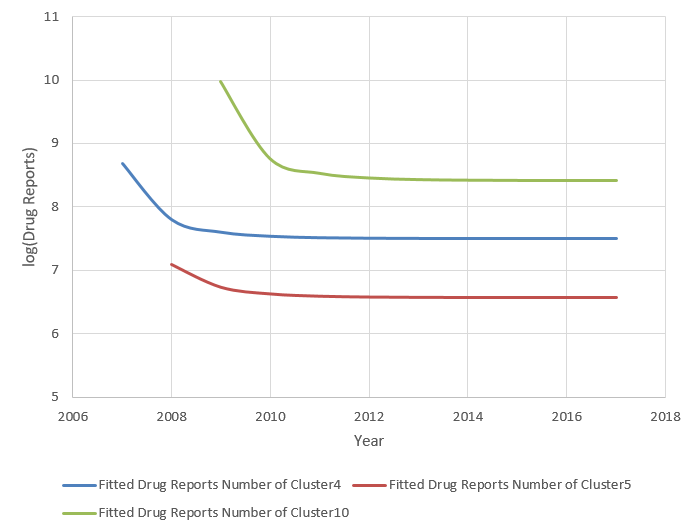
\includegraphics[scale=0.6]{./figures/1.png}
% 	\caption{Total Drug Reports Curves of Unsuitable Clusters}
% 	\label{Fig.1}
% \end{figure}

According to fitted curves of the remaining data, we obtain the curves of drug-use level for 20 years from 2000 to present. Then, we look for intersections of every curve and the time axis. Fig. \ref{Fig.2} describes most clusters’ characteristics of total drug use.

We can clearly see that Cluster-2, where drug cases have started since 1999, is earlier than any other six clusters and this is exactly our target to find in specific opioids in most clusters.

Therefore, we further make use of this model to analyze the usage of heroin and synthetic opioids screened in data screening and acquire the following results.

\begin{figure}[H]
	\centering %图片全局居中
	%并排几个图,就要写几个minipage
	\begin{minipage}[b]{0.45\textwidth} %所有minipage宽度之和要小于1,否则会自动变成竖排
		\centering %图片局部居中
		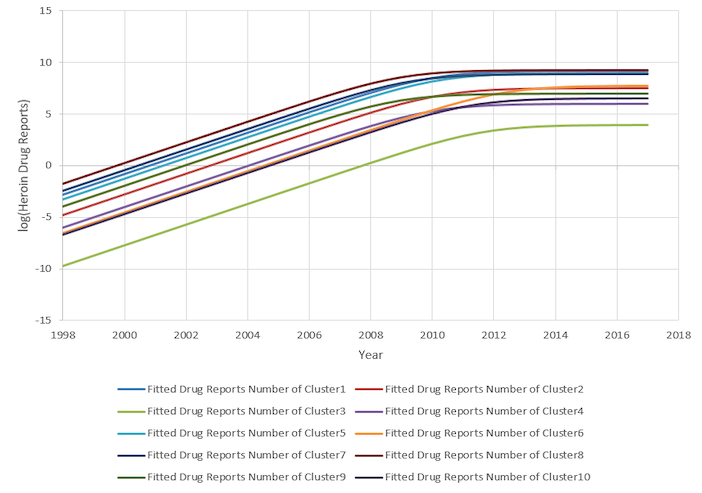
\includegraphics[scale=0.39]{./figures/3.png} %此时的图片宽度比例是相对于这个minipage的,不是全局
		\caption{Drug Reports for Heroin}
		\label{Fig.3}
	\end{minipage}
	\begin{minipage}[b]{0.45\textwidth} %所有minipage宽度之和要小于1,否则会自动变成竖排
		\centering %图片局部居中
		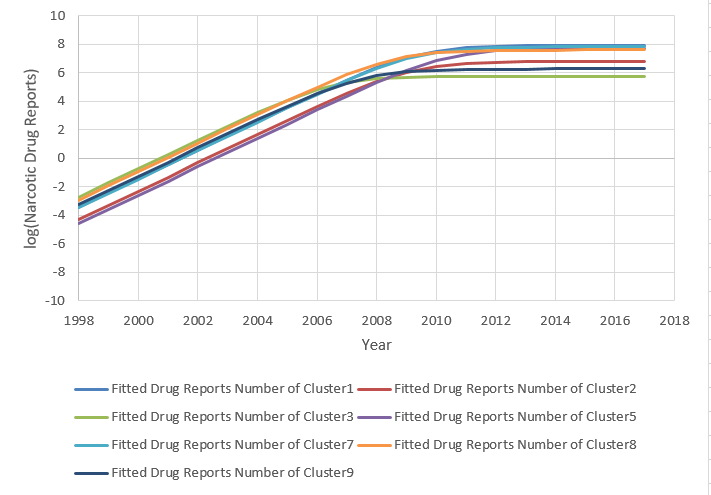
\includegraphics[scale=0.5]{./figures/4.png}%此时的图片宽度比例是相对于这个minipage的,不是全局
		\caption{Drug Reports for Syntheic Opioids}
		\label{Fig.4}
	\end{minipage}
\end{figure}

As we can see from Fig. \ref{Fig.3}, the Cluster-8 in the ten clusters has already started using heroin drugs before 2000. It can be considered that counties which belongs to Cluster-8 could be the locations where heroin started to appear and use.

In Fig. \ref{Fig.4}, it can be seen that Cluster-1, 3, 7, 8, and 9 all started using drugs around 2001. Because the time accuracy is not particularly precise, they may all be the areas where synthetic opioids were used earlier. According to our model, we believe that the TODO represented by Cluster-3 is the area where the synthetic opioids use have started earlier, and the other TODO represented by other clusters(Cluster-1,7,8 and 9) may also be areas that have already been used.

What’s more, we use the logistic discrete equation to solve the coefficients of the regression, and obtain the maximum tolerance of drug-use in each region based on this model. Results presented presented in the following table will continue to be used in subsequent models.

\subsection{Iterative Lokta-Voltera Model to describe the spread and characteristics}
In the last section 4.1, we construct Logistic Model to identify the possible locations where specific opioid use might have started. However, as the number of drug reports approaches the carrying capacity $N_{max}$, the Logistic Model become smooth and can’t provide more information about the changing trends. Therefore, in this section, we modify the dynamic Lotka-Volterra equations to model the interactions between different clusters.
	
The Lotka-Volterra equations are known as the predator-prey equations in a biological system of two (or more) species. In fact, the Lotka-Volterra equations can describe not only the predation relationships between species, but also the competition, parasitism even mutualism relationships. And we think the spread of the reported synthetic opioid and heroin incidents may have a mixed features, which meets the application conditions.

For simplification, let $S_{1}$ and $S_{2}$ denote, respectively, Species 1 and Species 2. Let $u_{1}(t)$ and $u_{2}(t)$ denote, respectively, the measurement of $S_{1}$ and $S_{2}$ at time t. Let $a_{1}$ and $a_{2}$ denote the natural growth fate of $S_{1}$ and $S_{2}$, and $b_{1}$ and $b_{2}$, respectively, the influence factor of $S_{1}$ to the natural growth rate of $S_{1}$ and $S_{2}$. Similarly, here goes the $c_{1}$ and $c_{2}$. The Lotka-Voltera equations are non-linear, first-order differential equations defined as follows:
\begin{gather}
	u'_{1}(t) = u_{1}(t)(a_{1} + b_{1}u_{1}(t) + c_{1}u_{2}(t)) \label{equ41}\\
	u'_{2}(t) = u_{2}(t)(a_{2} + b_{2}u_{2}(t) + c_{2}u_{2}(t))
\end{gather}

Next, we extend and apply the above equations to model interactions between the 10 clusters. Let $u_{k}(t)$ denote the Cluster-k, where k = 1,2,…,10. Let $a_{k}$ denote the change rate of Cluster-k itself, and $b_{kj}$ denote the influence of Cluster-j to Cluster-k. The equations can be written as
\begin{equation}
	\begin{split}
	\frac{du_{k}(t)}{dt} &= u_{k}(t)(a_{k} + \sum_{j=1}^{9}b_{kj}u_{k}(t)) \\
	k &= 1,2,..,9
	\end{split}
\end{equation}

\begin{equation}
	\begin{pmatrix}
		\frac{du_{1}(t)}{dt} \\
		\frac{du_{2}(t)}{dt} \\
		\vdots \\
		\frac{du_{9}(t)}{dt}	
	\end{pmatrix}
	=
	\begin{pmatrix}
		u_{1}(t) \\
		u_{2}(t) \\
		\vdots \\
		u_{9}(t)
	\end{pmatrix}
	\otimes
	\begin{pmatrix}
		a_{1} & b_{11} & \ldots & b_{19}\\
		\vdots & \vdots & \ddots & \vdots\\
		a_{9} & b_{91} & \ldots & b_{99}
	\end{pmatrix}
	\ast
	\begin{pmatrix}
		1 \\
		u_{1}(t) \\
		u_{2}(t) \\
		\vdots \\
		u_{9}(t)
	\end{pmatrix}
\end{equation}

For the ease of calculation and prediction, we modify the equation as follows. Let $\bm{\bar U(t)}$ denote the vector $\bm{[du_{k}(t)/dt]^{T}_{1*n}}$  , $\bm{U(t)}$ denote the vector $\bm{[u_{k}(t)]^{T}_{1*n}}$  , $\bm{A}$ denote the matrix $\bm{[\bar a | {\bar B}]}$ where $\bm{{\bar a}=[a_{k}]^T_{1*n}}$  , $\bm{{\bar B}=[b_{kj}]_{n*n}}$.
\begin{equation}
	\bm {{\bar U(t)}=U(t)\otimes A \times [1 | U(t)^{T}]^{T}}
\end{equation}

We notice the time parameter is discrete. In order to make the equation iterated, we transformed equations as follows:
\begin{equation}
	\begin{pmatrix}
		\frac{1}{u_{1}(t)}\frac{du_{1}(t+1)}{dt} \\
		\frac{2}{u_{2}(t)}\frac{du_{2}(t+1)}{dt} \\
		\vdots \\
		\frac{3}{u_{3}(t)}\frac{du_{3}(t+1)}{dt}	
	\end{pmatrix}
	=
	\begin{pmatrix}
		\frac{u_{1}(t+1)}{u_{1}(t)} - 1 \\
		\frac{u_{2}(t+1)}{u_{2}(t)} - 1 \\
		\vdots \\
		\frac{u_{9}(t+1)}{u_{9}(t)} - 1
	\end{pmatrix}
	=
	\begin{pmatrix}
		a_{1} & b_{11} & \ldots & b_{19} \\
		\vdots & \vdots & \ddots & \vdots \\
		a_{9} & b_{91} & \ldots & b_{99}
	\end{pmatrix}
	\ast
	\begin{pmatrix}
		1 \\
		u_{1}(t) \\
		u_{2}(t) \\
		\vdots \\
		u_{9}(t)
	\end{pmatrix}
\end{equation}

\begin{equation}
	\begin{pmatrix}
		\frac{u_{1}(t+1)}{u_{1}(t)} \\
		\frac{u_{2}(t+1)}{u_{2}(t)} \\
		\vdots \\
		\frac{u_{9}(t+1)}{u_{9}(t)} \\
	\end{pmatrix}
	=
	\begin{pmatrix}
		a_{1} & b_{11} & \ldots & b_{19} \\
		\vdots & \vdots & \ddots & \vdots \\
		a_{9} & b_{91} & \ldots & b_{99}
	\end{pmatrix}
	\ast
	\begin{pmatrix}
		1 \\
		u_{1}(t) \\
		u_{2}(t) \\
		\vdots \\
		u_{9}(t)
	\end{pmatrix}
	+
	\begin{pmatrix}
		1 \\
		1 \\
		\vdots \\
		1
	\end{pmatrix}
\end{equation}

\begin{equation}
	\begin{pmatrix}
		u_{1}(t+1) \\
		u_{2}(t+1)\\
		\vdots \\
		u_{9}(t+1) \\
	\end{pmatrix}
	=
	\begin{pmatrix}
		u_{1}(t) \\
		u_{2}(t) \\
		\vdots \\
		u_{9}(t)
	\end{pmatrix}
	\otimes 
	\left \{
	\begin{pmatrix}
		a_{1} & b_{11} & \ldots & b_{19} \\
		\vdots & \vdots & \ddots & \vdots \\
		a_{9} & b_{91} & \ldots & b_{99}
	\end{pmatrix}	
	\ast
	\begin{pmatrix}
		1 \\
		u_{1}(t) \\
		u_{2}(t) \\
		\vdots \\
		u_{9}(t)
	\end{pmatrix}
	+
	\begin{pmatrix}
		1 \\
		1 \\
		\vdots \\
		1
	\end{pmatrix}
	\right \}
\end{equation}

And we get the final iterative equation as follows:
\begin{equation}
	\bm{U(t+1) = U(t)} \otimes \{\bm{A * [1 | U(t)}^{T}]^{T} + 9 * [1]\} = \bm{g(U(t))}
\end{equation}

In order to get the iterative matrix $\bm{A}$, we use the least square method to estimate. For Cluster-i, the vector $[a_{i}, b_{i1}, ..., b_{i9}]$ has 10 parameters, while we only have 8 equations ranging from 2010 to 2017, which can’t meet the condition of least square $n > k$ . Therefore, we use the interpolation method to increase sample points. For simplicity, we take the median of any two adjacent sample points as the interpolation value.

\begin{equation}
	\bm{U}(\bm{t}+\frac{1}{2}) = \cfrac{\bm{U}(\bm{t}+1) + \bm{U}(\bm{t})}{2}
\end{equation}

Fig. \ref{Fig5} depicts the trend of opioid and heroin incidents in the 10 clusters for the next 7 years.
\begin{figure}[H]
	\centering
	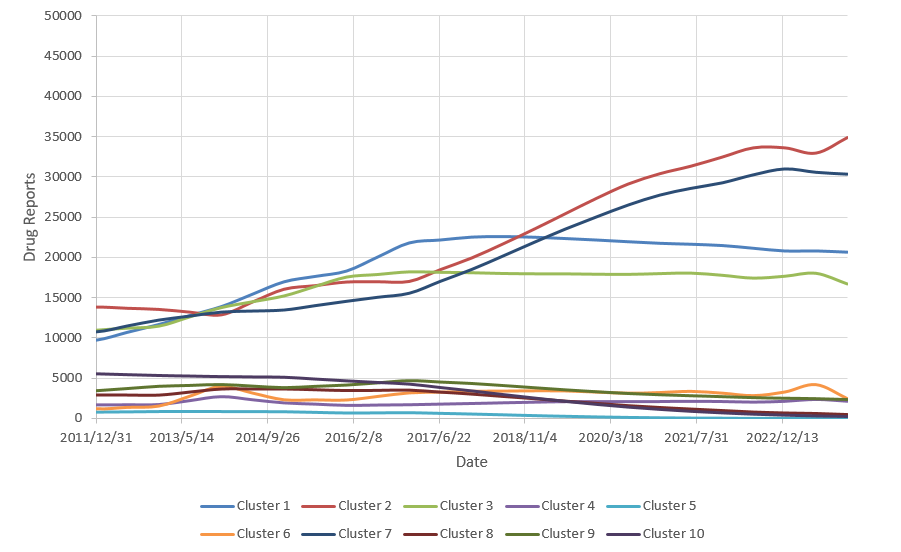
\includegraphics[scale=0.5]{./figures/5.png}
	\caption{Trend of the Next 5 Years}
	\label{Fig5}
\end{figure}

According to the logistic model, we have obtained tolerances for drug-use levels in each region, which we approximately consider as the drug threshold level for each region, making an analogy with the maximum environmental capacity in biology. If drug usage exceeds the threshold level, the trend of drug use in this region will be uncontrollable and may create an unpredictable social crisis.

In the above figure, we know that the trend of drug use in some areas is decreasing year by year or stable at a relatively low value. So it can be considered that the drug usage will not exceed its threshold level for the next few years, and the government does not need to worry about these areas. Here we will no longer make these curves. Now we need to study several clusters with clearly upward trends, and we need to find the intersection of the drug threshold level and the rising curve in order to make a judgement about whether government should take actions. The following figures also clearly reflect this feature.

We can see that both Cluster-2 and 7 exceed the drug threshold levels. Cluster 2 will reach the threshold level 2018, which is said that government should take measures as much as quickly to prevent this area’s problems. And Cluster-7 will reach the level few years later, around 2021. Also, it shows that their trends in the following years are still increasing. At this time, it can be considered that drug use may be uncontrolled in these two regions when the levels are exceeded. Thus, the government needs to adopt measures in advance and pay attention to the growth of drug use levels in these two areas earlier.

\begin{figure}[H]
	\centering %图片全局居中
	%并排几个图,就要写几个minipage
	\begin{minipage}[b]{0.45\textwidth} %所有minipage宽度之和要小于1,否则会自动变成竖排
		\centering %图片局部居中
		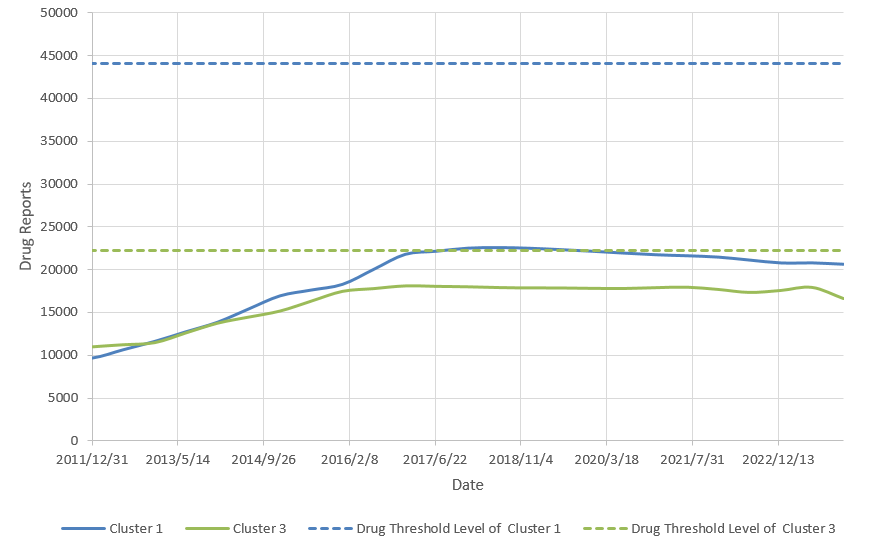
\includegraphics[scale=0.37]{./figures/6.png} %此时的图片宽度比例是相对于这个minipage的,不是全局
		\caption{Threshold levesl of Cluster-1 and Cluster-3}
		\label{Fig6}
	\end{minipage}
	\begin{minipage}[b]{0.45\textwidth} %所有minipage宽度之和要小于1,否则会自动变成竖排
		\centering %图片局部居中
		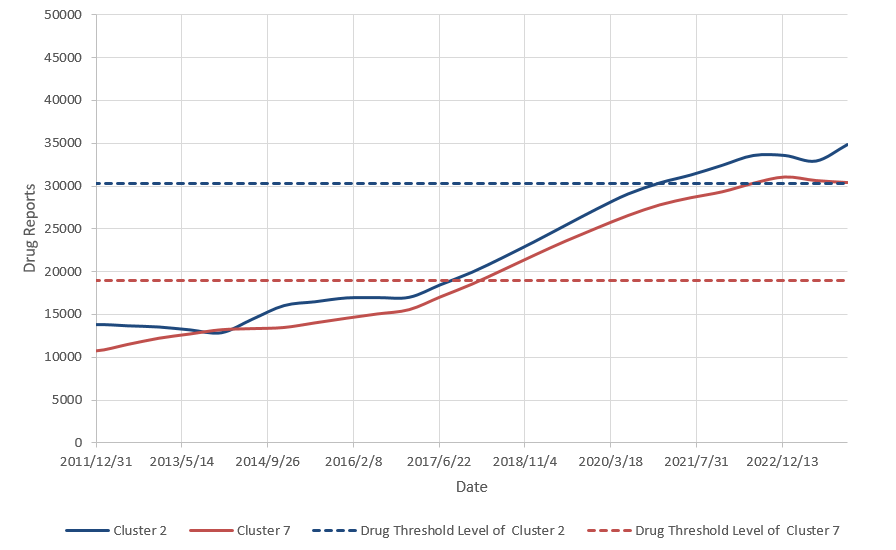
\includegraphics[scale=0.37]{./figures/7.png}%此时的图片宽度比例是相对于这个minipage的,不是全局
		\caption{Threshold Levels of Cluster-2 and Cluster-7}
		\label{Fig7}
	\end{minipage}
\end{figure}


However, the Modified Lotka-Volterra Model we construct is an unstable differential equations. As time goes on, the differential equations system show chaotic phenomena. Every 20 years, all the values of 10 clusters fluctuate severely and then suddenly converge to 0. Fig. \ref{Fig8} depicts the trend of opioid and heroin incidents in the 10 clusters for the next 50 years.
\begin{figure}[H]
	\centering
	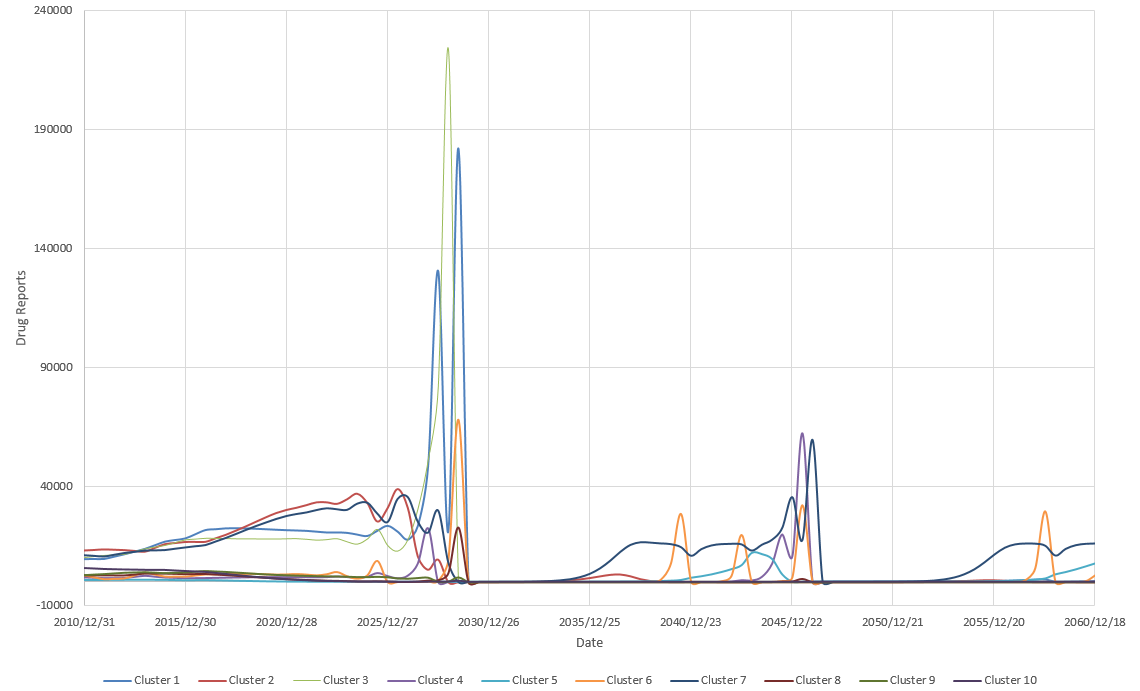
\includegraphics[scale=0.5]{./figures/8.png}
	\caption{Trend of the Next 50 Years}
	\label{Fig8}
\end{figure}

The reasons for the model failure are as follows:
\begin{enumerate}
	\item We use the least square method to estimate the iterative matrix A by samples from 2010 to 2017. However, in the reality, the interactions between different clusters may change with time. \item The patterns and characteristics we derive from samples may continue only for s short time.
	For Equation \ref{equ41}, we set the right-hand side of the system to 0, to get 4 equilibrium points
\end{enumerate}
\begin{gather*}
	A_{1}(0, 0) \\
	A_{2}(0, \frac{c_{1}a_{2}-a_{1}c_{2}}{b_{1}c_{2}-c_{1}b_{2}}) \\
	A_{3}(\frac{b_{1}a_{2} - a_{1}b_{2}}{c_{1}b_{2}-b_{1}c_{2}}, 0) \\
	A_{4}(\frac{b_{1}a_{2} - a_{1}b_{2}}{c_{1}b_{2}-b_{1}c_{2}}, \frac{c_{1}a_{2}-a_{1}c_{2}}{b_{1}c_{2}-c_{1}b_{2}}) 
\end{gather*}

The first three equilibrium points contain the coordinate 0, however each species shouldn’t extinct, which is inconsistent with reality. The reasonable equilibrium point $A_{4}$ should meet the conditions:
\begin{gather*}
	\left \vert 
	\begin{matrix}
		a_{1} & a_{2} \\
		c_{1} & c_{2} 
	\end{matrix}
	\right \vert
	\ast
	\left \vert
	\begin{matrix}
		c_{1} & c_{2} \\
		b_{1} & b_{2}
	\end{matrix}
	\right \vert
	> 0 \\
	\left \vert 
	\begin{matrix}
		a_{1} & a_{2} \\
		b_{1} & b_{2} 
	\end{matrix}
	\right \vert
	\ast
	\left \vert
	\begin{matrix}
		b_{1} & b_{2} \\
		c_{1} & c_{2}
	\end{matrix}
	\right \vert
	> 0
\end{gather*}

The matrix $\bar B$ may not satisfy the corresponding conditions.

\section{Strengths and Weaknesses}
\subsection{Strengths}
\begin{itemize}
    \item Our model takes the idea of clustering, which overcomes the disadvantages of analysing either the whole state or one single county.
    \item We take several measures to process the dataset and make it convenient for use, while the authenticity and integrity of data is still maintained.
\end{itemize}

\subsection{Weaknesses}
\begin{itemize}
    \item Nothing yet
 \end{itemize}

\begin{thebibliography}{99}
\addcontentsline{toc}{section}{References}  %引用部分标题("Refenrence")的重命名
\bibitem{1}MacQueen, J. (1967, June). Some methods for classification and analysis of multivariate observations. In Proceedings of the fifth Berkeley symposium on mathematical statistics and probability (Vol. 1, No. 14, pp. 281-297).
\bibitem{2}Gazetteer Files - Geography - U.S. Census Bureau. \texttt{\\https://www.census.gov/geo/maps-data/data/gazetteer.html}
\bibitem{3}Shannon, C. E. (1948). A mathematical theory of communication. Bell system technical journal, 27(3), 379-423.
\bibitem{4}DrugBank. \texttt{https://www.drugbank.ca/drug}
\end{thebibliography}


% ==============以下为附录内容,如您的论文中不需要程序附录请自行删除====================
\clearpage
\begin{subappendices}						% 附录环境
\section*{Apendix: The Source Codes}		% 附录标题可以自行修改
\addcontentsline{toc}{section}{Appendix}  	% 将附录内容加入到目录中

This python program implements k-means clustering.
\lstinputlisting[language={python}, caption=\texttt{k-means.py}]{../code/k-means.py}
% \inputpython{../code/k-means.py}{0}{68}

This MATLAB program is used to calculate the value of variable $a$.
\begin{lstlisting}[language={Matlab}, caption=\texttt{temp.m}]
a = 0;
for i = 1:5
	a = a + 1;
end
\end{lstlisting}

This LINGO program is used to search the optimize solution of 0-1 problem.
\begin{lstlisting}[language=Lingo, caption=\texttt{temp.lg4}]
model:
sets:
WP/1..12/: M, W, X;
endsets
data:
M = 2 5 18 3 2 5 10 4 11 7 14 6;
W = 5 10 13 4 3 11 13 10 8 16 7 4;
enddata
max = @sum(WP:W*X);
@sum(WP: M * X)<=46;
@for(WP: @bin(X));
end
\end{lstlisting}

\textbf{\textcolor[rgb]{0.98,0.00,0.00}{Input matlab source:}}
% \lstinputlisting[language=Matlab]{../code/matlab-test.m}

\end{subappendices}
% =================================================================================



\end{document}